%%%%%%%%%%%%%%%%%%%%%%%%%%%%%%%%%%%%%%%%%
% Kieker Analysis Component
% 
% $Date$
% $Rev$:
% $Author$


\chapter{\KiekerAnalysisPart{} Component}\label{chap:componentsAnalysis}

\section{Analysis Controller and Pipe-And-Filter Framework}\label{sec:analysis:controller}

An analysis with \KiekerAnalysisPart{} is set up and executed employing %
the class \class{AnalysisController}. %
\KiekerAnalysisPart{} provides a framework to define and execute pipe-and-filter %
architectures of analysis plugins, i.e., monitoring readers and analysis filters, %
as well as repositories. %
%  requires a monitoring reader %
% (Section~\ref{sec:analysis:reader}) and at least %
% one monitoring record consumer plugin (Section~\ref{sec:analysis:consumer}). %
% In addition to the monitoring record consumer plugin, %
% other analysis plugins can be registered. %
Figure~\ref{fig:analysisController:classdiagram} shows the class diagram %
with the important \KiekerAnalysisPart{} classes and their relationship. %

\begin{figure}[h]\centering
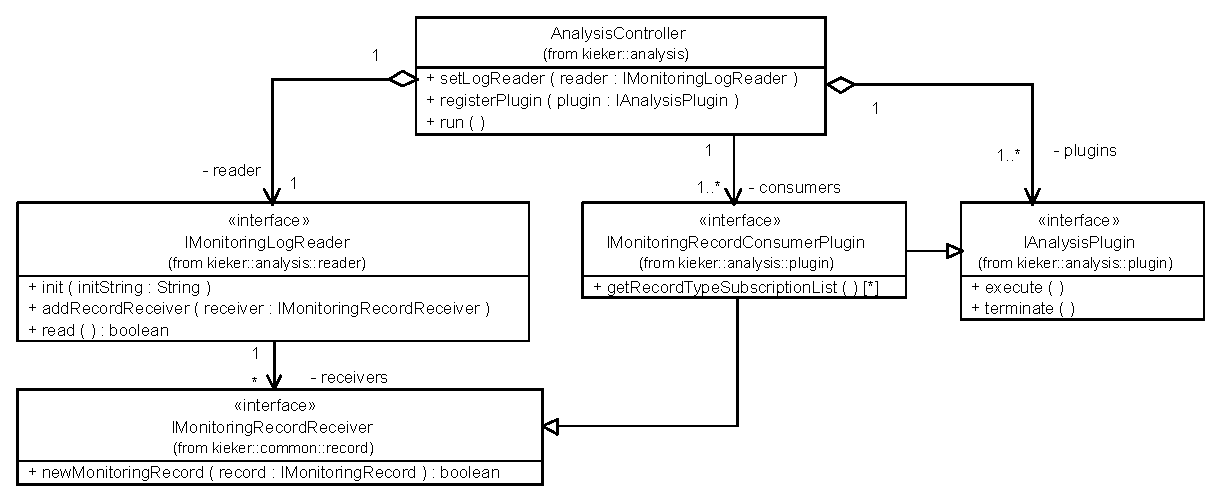
\includegraphics[scale=0.65]{images/kieker_AnalysisControlleruserguide-modified}
\caption{Class diagram showing important \KiekerAnalysisPart{} classes and their relationship}
\label{fig:analysisController:classdiagram}
\end{figure}

\noindent Setting up and running an analysis with \KiekerAnalysisPart{} requires the %
following steps to be performed, as described in Section~\ref{sec:example:analysis} already:\\

\enlargethispage{0.6cm}

\begin{compactenum}
\item Creating an instance of the \class{AnalysisController} class
\item Creating and registering monitoring readers (\method{registerReader}), 
filters (\method{registerFilter}), and repositories (\method{registerRepository}).
\item Connecting plugins and repositories (\method{registerRepository})
\item Starting the analysis instance (\method{run}).
\end{compactenum}



\noindent On invocation of the \method{run} method, the \class{Analysis Controller} %
calls the \method{init} method of all filter plugins allowing them to initialize. %
Then, it starts the configured monitoring readers by calling its \method{read} %
method. Plugins send data via their output ports to connected input ports of other 
plugins. As soon as the reader returns from the execution of its \method{read} 
method, the method \method{terminate} of each registered plugin is called by the %
\class{Analysis Controller}. %
In order to support the asynchronous execution of the \class{AnalysisController} instance, %
we provide the \class{AnalysisControllerThread} class.

\begin{figure}
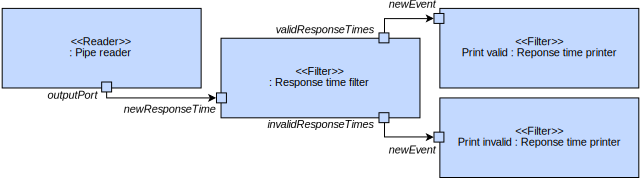
\includegraphics[width=\textwidth]{images/example-pipe-and-filter}
\caption{Example pipe-and-filter configuration}
\label{fig:example:pipe-and-filter}
\end{figure}


The remainder of this chapter describes how to develop custom reader and filter 
plugins, as well as repositories. The description is based on the example %
pipe-and-filter architecture shown in Figure~\ref{fig:example:pipe-and-filter}. The custom monitoring reader %
\class{MyPipeReader}, which corresponds to the writer developed in Section~\ref{sec:monitoring-log-writers}, %
sends records to the connected custom filter \class{MyResponseTimeFilter}. %
This filter accepts only events of the record type \class{MyResponseTimeRecord}, 
developed in Section~\ref{sec:componentsMonitoring:monitoringRecords}. %
The \class{MyResponseTimeFilter} classifies incoming \class{MyResponseTimeRecord}s %
based on whether they satisfy or exceed a configured threshold and pass them %
to the respective output ports, \method{validResponseTimes} or \method{invalidResponseTimes}. %
Two instances of a second custom filter, \class{MyResponseTimeOutputPrinter}, %
print the received records to the standard output stream.

\

\NOTIFYBOX{The Java sources of this chapter, as well as a pre-compiled binary, %
can be found in the %
\file{\customComponentsBookstoreApplicationDirDistro{}/} directory of the %
binary release.}

% The following Listing~\ref{listing:AnalysisController} shows how to create and run an analysis %
% with these custom components:
% 
% \setJavaCodeListing
% \lstinputlisting[caption=Code snippet setting up and running a \KiekerAnalysisPart{} instance (Starter.java),label=listing:AnalysisController,firstline=48, lastline=82, firstnumber=48]%
% {\customComponentsBookstoreApplicationDir/src/kieker/examples/userguide/ch3and4bookstore/Starter.java}

% \enlargethispage{1.2cm}

\section{Analysis Plugins}\label{sec:analysis:plugins}

Kieker analyis plugins are either monitoring readers, as detailed in Section~\ref{sec:analysis:reader}, %
or filters, as detailed in Section~\ref{sec:analysis:filters}. When implementing %
any of these two plugin types, the classes \class{AbstractReaderPlugin} or, %
respectively, \class{AbstractFilterPlugin} need to be extended (Figure~\ref{fig:analysisController:classdiagram}). %
Sections~\ref{sec:analysis:pluginAnnotation} and~\ref{sec:analysis:configuration} %
describe how to declare meta-information for plugins and the way to use %
configuration properties. To give a first impression of the programmatic %
instantiation, configuration, and connection of plugins, Listing~\ref{listing:StarterInitConnect} %
demonstrates this procedure for the example, using \class{MyPipeReader} and %
\class{MyResponseTimeFilter}, according to Figure~\ref{fig:example:pipe-and-filter}.

\setJavaCodeListing
\lstinputlisting[caption=Initializing and connecting the example reader and filter (Starter.java),label=listing:StarterInitConnect,firstline=53, lastline=68, firstnumber=53]%
{\customComponentsBookstoreApplicationDir/src/kieker/examples/userguide/ch3and4bookstore/Starter.java}

% The monitoring record consumer plugins described in the following %
% Section~\ref{sec:analysis:consumer}, are special analysis plugins that receive %
% the monitoring records provided by the monitoring reader. %
% Starting with these monitoring record plugins, analysis plugins can be connected %
% in a pipe-and-filter style to implement more complex analyses. %
% \Kieker{} provides input and output port interfaces and implementing classes %
% to implement such analyses. See the documentation of the classes \class{AbstractInputPort} %
% and \class{OutputPort} for details. \KiekerTraceAnalysis{} is implemented %
% based on this pattern. 

\subsection{@Plugin Annotation and Output Ports}\label{sec:analysis:pluginAnnotation}

\noindent The \class{@Plugin} class annotation is used to define a %
plugin name, a description, and the list of output ports. %
Listing~\ref{listing:MyResponseTimeFilterPluginAnnotationOutputs} shows the %
\class{@Plugin} annotation for the example filter.

If the \class{@Plugin} annotation is not present for a plugin, the \method{name} %
defaults to the plugin's (simple) classname, the \method{description} defaults %
to the empty string, and the list of output ports is empty. These default values %
are also used in case a respective attribute is omitted. %
Note that the name is not required to be a unique name for filters; it is simply %
used for descriptive purposes, such as in Figure~\ref{fig:example:pipe-and-filter}. %

Output ports are specified using the nested \class{@OutputPort} annotation. %
In addition to a name and a description for the output port, a list of event %
types can be specified. Note that in this case, the name is mandatory and must %
be unique for a plugin, as it is used for connecting input and output ports. %
The list of event types defaults to a list including only \class{Object.class}. %
The output port names should be provided as a \class{public static} constant %
with prefix \method{OUTPUT\_PORT\_NAME\_}, in order to ease the programmatic connection of %
pipe-and-filter, as previously shown in Listing~\ref{lst:BookstoreAnalysisStarter}.

\setJavaCodeListing
\lstinputlisting[firstline=31, firstnumber=31, lastline=44, caption={@Plugin annotation for the example plugin \class{MyResponseTimeFilter}}, label=listing:MyResponseTimeFilterPluginAnnotationOutputs]%
{\customComponentsBookstoreApplicationDir/src/kieker/examples/userguide/ch3and4bookstore/MyResponseTimeFilter.java}

\noindent Plugins can send events to their output ports by the \method{deliver} method %
provided by the super class. The method expects the output port name and %
the event to be sent as arguments. Listing~\ref{listing:MyResponseTimeFilterPluginAnnotationOutputs} %
shows how the example filter plugin \class{MyResponseTimeFilter} delivers records %
to its two output ports declared in the \class{@Plugin} annotation.

\setJavaCodeListing
\lstinputlisting[firstline=61, firstnumber=61, lastline=67, caption={Plugin sending events to output ports}, label=listing:MyResponseTimeFilterPluginAnnotationOutputs]%
{\customComponentsBookstoreApplicationDir/src/kieker/examples/userguide/ch3and4bookstore/MyResponseTimeFilter.java}

\subsection{Configuration}\label{sec:analysis:configuration}

\noindent According to the %
configuration of the \KiekerMonitoringPart{} components (see Section~\ref{sec:monitoring:configuration}), 
filters are configured via \class{Configuration} objects. Filters must %
provide a public constructor, accepting a \class{Configuration} object as %
its only argument. It is important to invoke the constructor of the super class. %
The configuration properties accepted by a plugin should be provided via \class{public static} %
constants with prefix \method{CONFIG\_PROPERTY\_NAME\_} in order to ease the %
programmatic initialization of plugins. For the example filter \class{MyResponseTimeFilter},
Listing~\ref{listing:MyResponseTimeFilterConstructor} shows the constructor, 
the configuration property and the corresponding member value obtained from the configuration.

\setJavaCodeListing
\lstinputlisting[firstline=45, firstnumber=45, lastline=53, caption={Plugin constructor with Configuration}, label=listing:MyResponseTimeFilterConstructor]%
{\customComponentsBookstoreApplicationDir/src/kieker/examples/userguide/ch3and4bookstore/MyResponseTimeFilter.java}

\noindent Additionally, filters must provide a default configuration and the %
current configuration via the methods \method{getDefaultConfiguration} and %
\method{getCurrentConfiguration}. Please note that the returned configuration %
must be sufficient to initialize the filter via the mentioned constructor. %
The \class{AnalysisController} uses the \method{getCurrentConfiguration} to %
save the pipe-and-filter configuration. Listing~\ref{listing:MyResponseTimeFilterEventsToOutput} %
shows how the methods are implemented for the example filter \class{MyResponseTimeFilter}. %

\setJavaCodeListing
\lstinputlisting[firstline=72, firstnumber=72, lastline=84, caption={Plugin returning its default and current configuration}, label=listing:MyResponseTimeFilterEventsToOutput]%
{\customComponentsBookstoreApplicationDir/src/kieker/examples/userguide/ch3and4bookstore/MyResponseTimeFilter.java}

\subsection{Monitoring Reader Plugins}\label{sec:analysis:reader}

% Warning-tag for the reader-writer-thing
The monitoring readers are the direct counterpart to the monitoring %
writers. While writers receive records and write them into files or other kinds %
of monitoring logs/streams, readers deserialize monitoring data and provide it as %
\class{IMonitoringRecord} instances. 

\begin{figure}[h]\centering
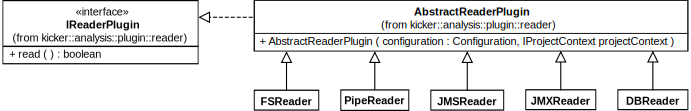
\includegraphics[scale=0.7]{images/kieker_readerimplsuserguide-modified}
\caption{Interface \class{IMonitoringReader} and implementing classes}
\label{Figure:ReaderHierarchy}
\end{figure}

% \pagebreak

% \
% 
% \WARNBOX{This means that whenever a new writer is implemented, a corresponding reader has to be implemented as well. If one want for example to store the recorded informations in a database, one should be capable of reading these saved informations from the database again.}
% 
% \

% \enlargethispage{1cm}

\noindent There are already some readers implemented in \Kieker,  as shown in the %
class diagram in Figure \ref{Figure:ReaderHierarchy}. %
The \class{FSReader} has already been used in Section~\ref{sec:example:analysis}. %
The \class{FSReaderRealtime} can be used to simulate continuous monitoring of a %
production system. It adds delays between the delivery of the monitoring records %
to its consumers according to the original delays reconstructed from the logging %
timestamps (Section~\ref{sec:componentsMonitoring:monitoringRecords}).
A brief description of how to use the \class{JMSReader} can be found in Appendix~\ref{appendix:usingJMS}. %

\noindent The implementation of a custom reader is similar to the implementation of a %
monitoring writer. Custom readers should extend the class \class{AbstractKiekerMonitoringReader} %
which already provides an implementation of the observer pattern. %
By invoking the method \method{deliverRecord},  the delivery of records is then %
delegated to the super class.

Listing~\ref{listing:MyReader} on page~\pageref{listing:MyReader} shows a simple reader which polls records from %
the named pipe introduced in the previous Chapter~\ref{chap:componentsMonitoring}. %

% If there is nothing on the pipe to be read, the reader waits 4 seconds at maximum before it terminates.
% \setJavaCodeListing
% \lstinputlisting[firstline=29, firstnumber=29, caption=MyPipeReader.java (excerpt), label=listing:MyReader,float]{\customComponentsBookstoreApplicationDir/src/kieker/examples/userguide/ch3and4bookstore/MyPipeReader.java}


\setJavaCodeListing
\lstinputlisting[firstline=30, firstnumber=30, lastline=38, caption={@Plugin annotation for the example reader}, label=listing:MyPipeReaderPluginAnnotation]%
{\customComponentsBookstoreApplicationDir/src/kieker/examples/userguide/ch3and4bookstore/MyPipeReader.java}

\setJavaCodeListing
\lstinputlisting[firstline=30, firstnumber=30, lastline=38, caption={Example reader's initialization method}, label=listing:MyPipeReaderInit]%
{\customComponentsBookstoreApplicationDir/src/kieker/examples/userguide/ch3and4bookstore/MyPipeReader.java}

\setJavaCodeListing
\lstinputlisting[firstline=66, firstnumber=66, lastline=84, caption={Example reader's \method{read} method}, label=listing:MyPipeReaderInit]%
{\customComponentsBookstoreApplicationDir/src/kieker/examples/userguide/ch3and4bookstore/MyPipeReader.java}

\TODO{\method{terminate}}

\subsection{Filter Plugins}\label{sec:analysis:filters}

\setJavaCodeListing
\lstinputlisting[firstline=57, firstnumber=57, lastline=61, caption={@InputPort annotation for the example plugin's input method}, label=listing:MyResponseTimeFilterEventsToOutput]%
{\customComponentsBookstoreApplicationDir/src/kieker/examples/userguide/ch3and4bookstore/MyResponseTimeFilter.java}

\subsection{Repositories}

\setJavaCodeListing
\lstinputlisting[firstline=57, firstnumber=57, lastline=61, caption={@Respository annotation for Kieker's system model repository}, label=listing:RepositoryAnnotation]%
{../../src/tools/kieker/tools/traceAnalysis/systemModel/repository/SystemModelRepository.java}

\setJavaCodeListing
\lstinputlisting[firstline=44, firstnumber=44, lastline=48, caption={Declaration of required repositories in the @Respository annotation}, label=listing:RepositoryRequirementDeclaration]%
{../../src/tools/kieker/tools/traceAnalysis/filter/AbstractTraceAnalysisFilter.java}

\setJavaCodeListing
\lstinputlisting[firstline=135, firstnumber=135, lastline=135, caption={Accessing a repository within in a plugin}, label=listing:RepositoryAccess]%
{../../src/tools/kieker/tools/traceAnalysis/filter/AbstractTraceAnalysisFilter.java}

\section{Monitoring Record Consumer Plugins}\label{sec:analysis:consumer}

As just mentioned, consumer plugins are special analysis plugins which receive %
the records provided by the monitoring reader and implement analyses or %
visualizations based on these records. %
Consumer plugins must implement the interface \class{IMonitoringRecordConsumerPlugin} %
(see Figure~\ref{fig:analysisController:classdiagram}). %
By implementing the \method{getRecordTypeSubscriptionList} method, a consumer plugin %
can specify the desired types of monitoring records to be received via the %
method \method{newMonitoringRecord}.

The custom consumer in Listing~\ref{lst:MyReponseTimeConsumer} on %
page~\pageref{lst:MyReponseTimeConsumer} simply writes %
the content of the received response time records to the standard output stream.

% \pagebreak
% \setJavaCodeListing
%\lstinputlisting[caption=MyReponseTimeConsumer.java,label=lst:MyReponseTimeConsumer,firstline=21,firstnumber=21]{\customComponentsBookstoreApplicationDir/src/kieker/examples/userguide/ch3and4bookstore/MyResponseTimeConsumer.java}
